\chapter{CP}
A common scientific pattern, usually used to better understand a problem, is to decompose the case into
simpler and simpler parts that take in account just one or few aspects of the problem.
When we can control those aspect with a certain amount of reliability, we can mix different parts in order to
ensure that the superposition of those effects behaves as expected.
In this way we can build incremental models, that solve the problem by looking and optimizing a certain aspect
if the problem. 

\section{Base Model}
The \textbf{Base Model} is the most basic, where we defined our problem view, such as the parameters and the variables,
and we decided how to constraint it in order to get a satisfiable solution:

\begin{center}
    \begin{adjustwidth}{-1.5cm}{}
        \begin{tabular}{|c|c|c|}
            \hline
            \multicolumn{3}{|c|}{\textbf{Parameters}} \\
            \hline
            \textbf{Parameter} & \multicolumn{2}{|c|}{\textbf{Description}} \\
            \hline
            Width & \multicolumn{2}{|c|}{The Paper Sheet Width} \\
            \hline
            Height & \multicolumn{2}{|c|}{The Paper Sheet Height} \\
            \hline
            Presents & \multicolumn{2}{|c|}{The number of the Presents to place in the Paper Sheet} \\
            \hline
            Dimension X & \multicolumn{2}{|c|}{The array of the x dimensions of the Presents} \\
            \hline
            Dimension Y & \multicolumn{2}{|c|}{The array of the y dimensions of the Presents} \\
            \hline
            \multicolumn{3}{|c|}{\textbf{Extracted Parameters}} \\
            \hline
            \textbf{Parameter} & \textbf{Formula} & \textbf{Description} \\
            \hline
            Area & $Area = Width \cdot Height$ & Area of the Paper \\
            \hline
            Areas & $Areas[i] = Dimension_x[i] \cdot Dimension_y[i]$ & The array of the areas of the Presents \\
            \hline
            \multicolumn{3}{|c|}{\textbf{Variables}} \\
            \hline
            \textbf{Variable} & \multicolumn{2}{|c|}{\textbf{Description}} \\
            \hline
            Coord X &  \multicolumn{2}{|c|}{Array of the X positions of each Present} \\
            \hline
            Coord Y &  \multicolumn{2}{|c|}{Array of the Y positions of each Present} \\
            \hline
        \end{tabular}
    \end{adjustwidth}
\end{center}


\subsection{Main Problem Constraints}
Once the description of the problem is carried out, we defined some general constraints
in order to instruct the way to find a solution to the solver. The constraints are:

\begin{itemize}
    \item[] \textbf{Essential Constraints}
    \item \textbf{\textit{The presents must fit into the Paper Sheet:}}
        \begin{itemize}
            \item[] A present fits in the paper if its coordinates are strictly positive
                and its coorinates summed with its corresponding dimensions are lesser then
                the Paper Sheet dimensions.
            \item[] The resultant constraint is:
            \item[] $\forall i \in [1, Presents] \rightarrow\\(Coord_x[i] + Dimension_x[i] \leq Width + 1) \wedge \\ (Coord_y[i] + Dimension_y[i] \leq Height + 1)$  
            \item[] \textit{As we used indexes starting from 1, we must add 1 to the right side of both disequations} 
        \end{itemize}

    \item \textbf{\textit{Two different presents must not overlap:}}
        \begin{itemize}
            \item[] Given the two rectangles of two different presents, we can check if they have
                at least one part in common, just by checking their corners. So, we defined the
                \textit{overlaps} predicate:
            \item[] $overlaps(
                Left^1_x, Right^1_x, Left^1_y, Right^1_y,
                Left^2_x, Right^2_x, Left^2_y, Right^2_y
                ) \leftrightarrow
                \neg (Left^1_x \geq Right^2_x \vee Left^2_x \geq Right^1_x) \wedge\\
                \neg (Right^1_y \leq Left^2_y \vee Right^2_y \leq Left^1_y)$
            \item[] Each present is described as the rectangle:
            \item[] $Left^i_x, Left^i_y, Right^i_x, Right^i_y$
            \item[] So we can constraint each couple of presents to not overlaps one to each other:
            \item[] $
            \forall i, j \in [1, Presents], j > i \rightarrow\\
                \neg overlaps(\\
                    Coord_x[i], Coord_x[i] + Dimension_x[i], Coord_y[i], Coord_y[i] + Dimension_y[i],\\
                    Coord_x[j], Coord_x[j] + Dimension_x[j], Coord_y[j], Coord_y[j] + Dimension_y[j]\\
                )$ 
        \end{itemize}

        \begin{figure}
            \centering
            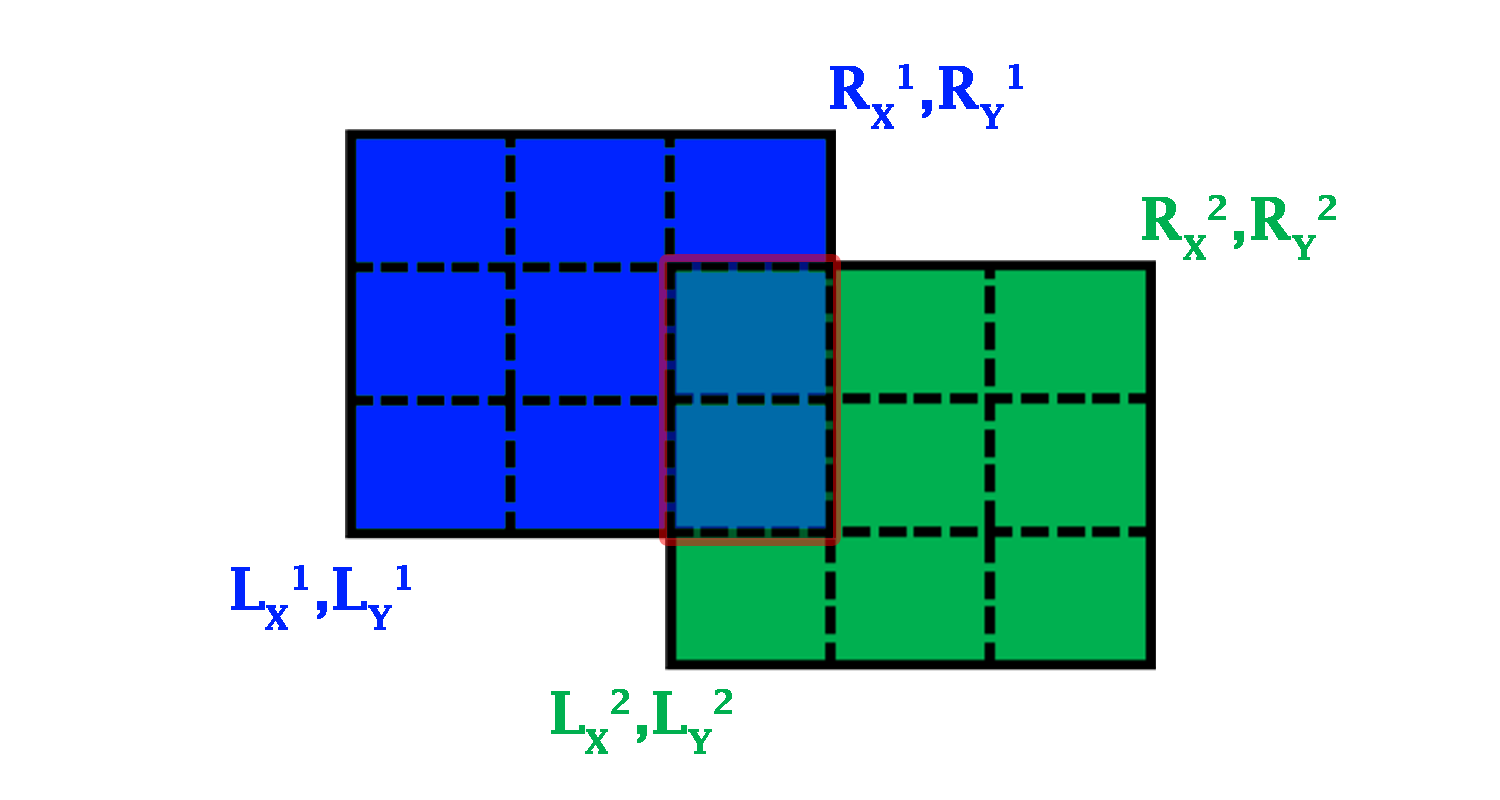
\includegraphics[width=\textwidth]{overlaps}
            \caption{Overlapping Model}
            \label{fig:overlaps}
        \end{figure}

    \item[] \textbf{Additional Constraints}
    \item[] These constraint are not essential to solve the general formulation of this problem,
        but they results helpful as they restrict the search space in the given instances.
        The underlying assumption is that the instance contains the right amount of presents such
        that the area of the Paper Sheet is completely used.
    \item \textbf{\textit{The total area of the presents must be the same of the Paper Sheet:}}
        \begin{itemize}
            \item[] $\sum_{i = 1}^{Presents}{Areas[i]} = Area$
            \item[] This constraint prevents the exploration of the search space
                at the very beginning. We indeed can instantly infer if the given instance is
                feasible: if the total areas does not match we can say the problem is unsatisfiable.
            \item[] A further relaxation of this constraint is to use $\leq$ instead of $=$ in order 
                to keep instances where we have presents that do not completely fill the Paper Sheet. 
                We kept the strict constraint for efficency reason, because the given instances all fall
                in this case.
        \end{itemize}
    \item \textbf{\textit{The presents must fill the row (column) dimension:}}
        \begin{itemize}
            \item[] As an extension of the previous constraint, we want to use each row \textit{(or column)}
                such that we use all of the available area of the paper.
            \item[] Drawing a vertical \textit{(horizontal)} line and summing up the encountered
                presents dimensions we must end up with the same dimension of the Paper Sheet:
            \item[] Rows: $
                \forall y \in [1, Height] \rightarrow\\ \sum_{i = 1}^{Presents}{
                    \begin{cases}
                    Dimension_x[i] & \text{if } y \geq Coord_y[i] \wedge y < Coord_y[i] + Dimension_y[i] \\
                    0 & \text{otherwise}
                    \end{cases}
                    }\\= Width$
            \item[] Columns: $
                \forall x \in [1, Width] \rightarrow\\ \sum_{i = 1}^{Presents}{
                    \begin{cases}
                    Dimension_y[i] & \text{if } x \geq Coord_x[i] \wedge x < Coord_x[i] + Dimension_x[i] \\
                    0 & \text{otherwise}
                    \end{cases}
                    }\\= Height$
        \end{itemize}
\end{itemize}

\subsection{Search Methods}
All of the constraints we described so far could solve the given instances with the \textit{Geocode} solver,
but the main difficulty is the time spent in the resolution. Some instances can take more then 10 minutes.
To lower the elasped time, we can tell to the solver how to optimize the search on the variables:
\begin{itemize}
    \item We decided to choose a preferential axes for the search. The X axis was choosen.
    \item Each axis then can be explored in different ways. We want to explore it with the most difficult case
        as we already know that some presents configurations can exclude a priori the placement of other presents.
        In this way we selected the \textit{\textbf{first\_fail}} search parameter, that chooses the variable with
        the smallest domain and try to find out if can have a value in the current solution state.
        If there are no possible values, we prevented the solver to search useless branch of the search tree.
        As we place presents into the sheet, each variable will lose a part of its domain, so we will choose that
        one that is most likely to fail.
    \item Now we must select an heuristic that chooses intelligently a value for the given variable. Our problem
        description has coordinates of each presents in their lower left corner, so we try to assign first the lesser
        available coordinates, then the bigger one. The \textit{\textbf{indomain\_min}} search parameter try to assign
        to each variable the minimum value available in the current domain.
    \item The final search annotiation is:
    \item[] $seq\_search([\\
            \text{\ \ \ \ }int\_search(Coord\_X, first\_fail, indomain\_min),\\
            \text{\ \ \ \ }int\_search(Coord\_Y, first\_fail, indomain\_min)\\
        ])$
\end{itemize} 

We also tried any combination of all the possible parameters in order to confirm our reasoning, so we end up by choosing
this setup because it resulted the most performant.


\begin{center}
    \begin{tabular}{|c|c|r|r|}
        \hline
        \multicolumn{4}{|c|}{\textbf{Results}} \\
        \hline
        \textbf{Instance} & \textbf{Time} & \textbf{Nodes} & \textbf{Propagations} \\
        
        \hline
		8x8 & 00:00:00.001 & 5 & 179 \\ \hline
		9x9 & 00:00:00.001 & 6 & 287 \\ \hline
		10x10 & 00:00:00.000 & 6 & 405 \\ \hline
		11x11 & 00:00:00.000 & 10 & 705 \\ \hline
		12x12 & 00:00:00.001 & 14 & 1,328 \\ \hline
		13x13 & 00:00:00.002 & 15 & 1,424 \\ \hline
		14x14 & 00:00:00.001 & 11 & 985 \\ \hline
		15x15 & 00:00:00.001 & 13 & 1,118 \\ \hline
		16x16 & 00:00:00.001 & 12 & 1,272 \\ \hline
		17x17 & 00:00:00.004 & 48 & 5,825 \\ \hline
		18x18 & 00:00:00.021 & 258 & 49,511 \\ \hline
		19x19 & 00:00:00.002 & 17 & 2,481 \\ \hline
		20x20 & 00:00:00.023 & 247 & 48,836 \\ \hline
		21x21 & 00:00:00.002 & 24 & 3,189 \\ \hline
		22x22 & 00:00:00.175 & 1,658 & 343,900 \\ \hline
		23x23 & 00:00:00.270 & 2,252 & 604,184 \\ \hline
		24x24 & 00:00:00.003 & 24 & 4,087 \\ \hline
		25x25 & 00:00:00.205 & 1,717 & 358,523 \\ \hline
		26x26 & 00:00:00.293 & 2,644 & 697,160 \\ \hline
		27x27 & 00:00:00.006 & 40 & 9,131 \\ \hline
		28x28 & 00:00:00.038 & 348 & 87,336 \\ \hline
		29x29 & 00:00:00.039 & 310 & 81,966 \\ \hline
		30x30 & 00:00:00.007 & 58 & 12,387 \\ \hline
		31x31 & 00:00:00.005 & 28 & 5,009 \\ \hline
		32x32 & 00:00:00.073 & 497 & 109,458 \\ \hline
		33x33 & 00:00:12.058 & 43,163 & 13,179,446 \\ \hline
		34x34 & 00:00:00.010 & 103 & 17,543 \\ \hline
		35x35 & 00:00:00.009 & 37 & 8,248 \\ \hline
		36x36 & 00:00:00.007 & 35 & 8,020 \\ \hline
		37x37 & 00:00:20.295 & 61,331 & 20,748,067 \\ \hline
		38x38 & 00:00:00.141 & 1,165 & 306,900 \\ \hline
		39x39 & 00:00:00.061 & 298 & 108,612 \\ \hline
		40x40 & 00:00:00.009 & 31 & 6,054 \\ \hline
		rotation\_test & - & - & - \\ \hline

    \end{tabular}
\end{center}


\section{Symmetry Model}
We had further analysed the problem in order to understand if, from an erroneous solution,
there are similar solutions that we can deduce as unsatisfiable as they are permutation or simmetrical of the
erroneous one. This technique is called \textbf{Symmetry Breaking}.\\
The \textbf{Present Wrapping Problem} \cite{project} is an extension of the \textbf{2D Bin Packing Problem},
and one of the most effective heuristic to place presents is to choose those that are more restricting for the others,
in other words, the bigger the present is, the most difficult is to place, the more it will restrict the other presents
domains and the more effective will be its placement in the first stages. So the best analytical and empirical heuristic
found so far for this kind of problem is to sort the presents in size order, placing the bigger first and the
smaller last \cite{binpack, algdesign}.\\
Doing this requires a new extracted parameter:

\begin{center}
    \begin{adjustwidth}{-1.5cm}{}
        \begin{tabular}{|c|c|c|}
            \hline
            \multicolumn{3}{|c|}{\textbf{Extracted Parameters}} \\
            \hline
            \textbf{Parameter} & \textbf{Formula} & \textbf{Description} \\
            \hline
            Sorted Areas Indexes & \makecell{$Sorted\_Areas\_Indexes =$ \\ $reverse(arg\_sort(Areas))$} & Indexes of the Areas sorted by Present Area \\
            \hline
        \end{tabular}
    \end{adjustwidth}
\end{center}

This new parameter stores the indexes of the sorted areas, so the $Sorted\_Areas\_Indexes[1]$ will store the indexes of the present with
the maximum area, $Sorted\_Areas\_Indexes[2]$ the index of the second present with maximum area and so on.\\
Now the most basic constraint we can add is that the biggest present will always stay on the minimal coordinates:\\
$
Coord\_X[Sorted\_Areas\_Indexes[1]] = 1\\
Coord\_Y[Sorted\_Areas\_Indexes[1]] = 1
$
\\

Then we want to place the bigger presents in the left-bottom most part of the paper, simulating the fact that we are placing them before
the others:\\
$
\forall i, j \in [1, Presents], j > i \rightarrow \\
    Coord_y[Sorted\_Areas_Indexes[i]] = Coord_y[Sorted\_Areas\_Indexes[j]] \rightarrow \\
    Coord_x[Sorted\_Areas_Indexes[i]] < Coord_x[Sorted\_Areas\_Indexes[j]]
$
\\
This, in combination with the search method, provides that the bigger present will be then the lesser will be its coordinate x,
and since the bigger the present, the smaller is its domain, it will be also placed first, that means in the lower y possible.
By doing this we can exclude all the possible symmetries due to the swap of different area presents.\\
Excluding the symmetrical solutions allow us to exclude also the symmetrical part of the search tree that are unsatisfiable, just
by finding an unsatisfiable combination out of the all simmetricals.

% TODO: Example Image


\begin{center}
    \begin{tabular}{|c|c|r|r|}
        \hline
        \multicolumn{4}{|c|}{\textbf{Results - CP - Symmetry Model}} \\
        \hline
        \textbf{Instance} & \textbf{Time} & \textbf{Nodes} & \textbf{Propagations} \\
        
        \hline
		8x8 & 00:00:00.001 & 3 & 150 \\ \hline
		9x9 & 00:00:00.001 & 5 & 357 \\ \hline
		10x10 & 00:00:00.003 & 5 & 461 \\ \hline
		11x11 & 00:00:00.001 & 10 & 1,265 \\ \hline
		12x12 & 00:00:00.007 & 45 & 8,116 \\ \hline
		13x13 & 00:00:00.004 & 11 & 2,159 \\ \hline
		14x14 & 00:00:00.001 & 19 & 2,599 \\ \hline
		15x15 & 00:00:00.011 & 142 & 27,081 \\ \hline
		16x16 & 00:00:00.002 & 9 & 1,814 \\ \hline
		17x17 & 00:00:00.011 & 80 & 24,551 \\ \hline
		18x18 & 00:00:00.003 & 26 & 5,218 \\ \hline
		19x19 & 00:00:00.039 & 316 & 91,564 \\ \hline
		20x20 & 00:00:00.099 & 536 & 123,172 \\ \hline
		21x21 & 00:00:00.192 & 900 & 304,328 \\ \hline
		22x22 & 00:00:00.125 & 544 & 190,132 \\ \hline
		23x23 & 00:00:06.933 & 19,260 & 9,171,901 \\ \hline
		24x24 & 00:00:00.371 & 1,488 & 638,669 \\ \hline
		25x25 & 00:00:03.943 & 12,490 & 4,788,188 \\ \hline
		26x26 & 00:00:01.367 & 3,595 & 2,087,114 \\ \hline
		27x27 & 00:00:02.178 & 4,784 & 3,049,562 \\ \hline
		28x28 & 00:00:16.155 & 43,295 & 23,048,023 \\ \hline
		29x29 & 00:00:05.314 & 15,069 & 11,628,851 \\ \hline
		30x30 & 00:00:00.046 & 287 & 100,741 \\ \hline
		31x31 & 00:00:00.135 & 916 & 301,542 \\ \hline
		32x32 & 00:00:00.148 & 387 & 267,579 \\ \hline
		33x33 & 00:00:00.350 & 1,580 & 770,610 \\ \hline
		34x34 & 00:00:00.471 & 1,701 & 827,950 \\ \hline
		35x35 & 00:00:00.410 & 1,752 & 935,117 \\ \hline
		36x36 & 00:00:04.800 & 14,412 & 8,047,884 \\ \hline
		37x37 & 00:00:39.646 & 93,562 & 45,084,879 \\ \hline
		38x38 & 00:00:01.475 & 6,150 & 2,711,326 \\ \hline
		39x39 & 00:00:04.727 & 16,581 & 10,166,321 \\ \hline
		40x40 & 00:00:02.233 & 7,408 & 3,362,652 \\ \hline
		rotation\_test & - & - & - \\ \hline

    \end{tabular}
\end{center}


\section{Rotation Model}
In a real life case we just know the two dimensions of each present we want to place, but we dont know in which order they should appear such that we can fit the paper sheet.
The rotation model can overwhelm this problem because it looks for any combination of rotated presents over the paper sheet, so we don't need to specify the right combination
of dimensions that can fit the paper. In order to do this, we need another variable in our description:

\begin{center}
		\begin{tabular}{|c|c|}
			\hline
			\multicolumn{2}{|c|}{\textbf{Variables}} \\
			\hline
			\textbf{Variable} & {\textbf{Description}} \\
			\hline
			Rotated & The boolean array that indicates whether a present is rotated or not \\
			\hline
		\end{tabular}
\end{center}

This variable keep trace of the rotation of the present. Keep in mind that in a discretized space, we can rotate a rectangular present just in two direction: $0\deg$ or $90\deg$.
Indeed if we further rotate the present, $180\deg$ for example, we end up with the non rotated present, or even more at $270\deg$ we obtain the $90\deg$ rotated present.
Thanks to their regularity of the geometric shape of the presents there are only two conditions of rotation, described by the inversion of the two dimensions.
To keep the problem description as simple as possible, we can just create a proxy function that returns the correct dimension depending on its rotation.
So if the present is not rotated, it return the right dimension, otherwise it will return the opposite dimension:\\
$
Get\_Dimension_x = 
\begin{cases}
	Dimension_y & \text{if } Rotated \\
	Dimension_x & \text{otherwise}
\end{cases}
$
\\
$
Get\_Dimension_y = 
\begin{cases}
	Dimension_x & \text{if } Rotated \\
	Dimension_y & \text{otherwise}
\end{cases}
$

Now, we can change any constraint that involves a dimension variable with the corresponding proxy.
In this way we obtained a model that can solve instances of the problem that are satisfiable only if we rotate one \textit{(or more)} present.


\begin{center}
    \begin{tabular}{|c|c|r|r|}
        \hline
        \multicolumn{4}{|c|}{\textbf{Results}} \\
        \hline
        \textbf{Instance} & \textbf{Time} & \textbf{Nodes} & \textbf{Propagations} \\
        
        \hline
		8x8 & 00:00:00.001 & 9 & 658 \\ \hline
		9x9 & 00:00:00.001 & 10 & 1,210 \\ \hline
		10x10 & 00:00:00.001 & 12 & 1,528 \\ \hline
		11x11 & 00:00:00.004 & 36 & 6,827 \\ \hline
		12x12 & 00:00:00.002 & 27 & 4,698 \\ \hline
		13x13 & 00:00:00.003 & 31 & 5,859 \\ \hline
		14x14 & 00:00:00.006 & 43 & 8,206 \\ \hline
		15x15 & 00:00:00.007 & 37 & 11,236 \\ \hline
		16x16 & 00:00:00.003 & 23 & 6,360 \\ \hline
		17x17 & 00:00:00.004 & 34 & 10,908 \\ \hline
		18x18 & 00:00:00.219 & 1,765 & 595,481 \\ \hline
		19x19 & 00:00:00.036 & 323 & 110,395 \\ \hline
		20x20 & 00:00:00.034 & 317 & 120,480 \\ \hline
		21x21 & 00:00:00.022 & 257 & 90,569 \\ \hline
		22x22 & 00:00:00.013 & 68 & 55,549 \\ \hline
		23x23 & 00:00:05.820 & 18,963 & 9,928,170 \\ \hline
		24x24 & 00:00:01.671 & 6,876 & 3,466,041 \\ \hline
		25x25 & 00:00:00.321 & 1,594 & 940,941 \\ \hline
		26x26 & 00:00:04.605 & 10,965 & 5,739,120 \\ \hline
		27x27 & 00:00:08.806 & 21,462 & 14,169,523 \\ \hline
		28x28 & 00:00:09.925 & 23,327 & 16,753,958 \\ \hline
		29x29 & 00:00:06.659 & 17,029 & 11,653,121 \\ \hline
		30x30 & 00:00:00.481 & 1,402 & 923,532 \\ \hline
		31x31 & 00:00:02.615 & 7,287 & 5,090,515 \\ \hline
		32x32 & 00:01:21.626 & 124,826 & 106,149,654 \\ \hline
		33x33 & 00:00:00.140 & 531 & 373,851 \\ \hline
		34x34 & 00:00:16.122 & 33,856 & 25,006,238 \\ \hline
		35x35 & 00:00:08.576 & 16,524 & 11,766,051 \\ \hline
		36x36 & 00:01:39.790 & 138,777 & 123,080,912 \\ \hline
		37x37 & 00:00:31.674 & 58,804 & 42,774,026 \\ \hline
		38x38 & 00:00:00.683 & 1,636 & 1,383,358 \\ \hline
		39x39 & 00:02:28.920 & 201,895 & 180,321,315 \\ \hline
		40x40 & 00:00:02.876 & 5,296 & 3,632,636 \\ \hline
		rotation\_test & 00:00:00.000 & 8 & 422 \\ \hline

    \end{tabular}
\end{center}


\section{Symmetry Rotation Model}
As we growth the model in modules, we can just combine the \textbf{Symmetry Model} with the \textbf{Rotation Model} and we end up
with a \textbf{Symmetry Rotation Model} that takes in account the possibility of the presents rotation and also excludes the symmetrical
solutions.


\begin{center}
    \begin{tabular}{|c|c|r|r|}
        \hline
        \multicolumn{4}{|c|}{\textbf{Results - CP - Rotation Symmetry Model}} \\
        \hline
        \textbf{Instance} & \textbf{Time} & \textbf{Nodes} & \textbf{Propagations} \\
        
        \hline
		8x8 & 00:00:00.001 & 6 & 617 \\ \hline
		9x9 & 00:00:00.001 & 8 & 1,209 \\ \hline
		10x10 & 00:00:00.004 & 9 & 1,614 \\ \hline
		11x11 & 00:00:00.002 & 15 & 3,303 \\ \hline
		12x12 & 00:00:00.020 & 98 & 41,544 \\ \hline
		13x13 & 00:00:00.006 & 29 & 9,686 \\ \hline
		14x14 & 00:00:00.007 & 25 & 8,707 \\ \hline
		15x15 & 00:00:00.016 & 67 & 36,917 \\ \hline
		16x16 & 00:00:00.005 & 18 & 6,954 \\ \hline
		17x17 & 00:00:00.054 & 172 & 144,085 \\ \hline
		18x18 & 00:00:06.256 & 16,229 & 10,835,714 \\ \hline
		19x19 & 00:00:00.072 & 343 & 177,304 \\ \hline
		20x20 & 00:00:00.072 & 216 & 155,813 \\ \hline
		21x21 & 00:00:00.092 & 282 & 171,238 \\ \hline
		22x22 & 00:00:00.089 & 142 & 120,023 \\ \hline
		23x23 & 00:00:50.231 & 84,786 & 67,222,960 \\ \hline
		24x24 & 00:00:02.629 & 4,305 & 3,829,157 \\ \hline
		25x25 & 00:00:01.636 & 3,268 & 2,502,639 \\ \hline
		26x26 & 00:00:16.392 & 25,167 & 20,198,711 \\ \hline
		27x27 & 00:01:15.713 & 92,814 & 98,743,399 \\ \hline
		28x28 & 00:00:09.897 & 11,008 & 12,137,938 \\ \hline
		29x29 & 00:00:13.392 & 20,629 & 22,838,424 \\ \hline
		30x30 & 00:00:00.409 & 679 & 696,482 \\ \hline
		31x31 & 00:00:05.386 & 10,221 & 8,993,129 \\ \hline
		32x32 & 00:01:49.602 & 116,283 & 151,800,684 \\ \hline
		33x33 & 00:00:01.136 & 1,704 & 2,066,471 \\ \hline
		34x34 & 00:00:34.985 & 40,978 & 45,436,467 \\ \hline
		35x35 & 00:00:12.991 & 18,472 & 19,219,173 \\ \hline
		36x36 & 00:03:32.730 & 217,539 & 265,720,097 \\ \hline
		37x37 & 00:00:42.944 & 56,905 & 61,576,669 \\ \hline
		38x38 & 00:00:00.863 & 1,660 & 1,812,527 \\ \hline
		39x39 & 01:14:47.299 & 7,970,705 & 9,871,119,474 \\ \hline
		40x40 & 00:00:35.196 & 48,956 & 52,211,662 \\ \hline
		rotation\_test & 00:00:00.000 & 4 & 377 \\ \hline

    \end{tabular}
\end{center}


\section{Duplicated Symmetry Model}
Another point to take in account, is the possibility of the presence of presents that have the same size. As we modelled the problem,
the \textbf{Base Model} can already solve this kind of instances, but we can add some constraints in order to exploit the \textbf{Symmetry Breaking}
even in these cases. The simpliest approach is to force the same size presents to be placed in the order they appear. In this way we put in the lesser
coordinates the presents that are in the first positions of the parameter $Dimension_X$ and $Dimension_y$ arrays:\\

$
\forall i, j \in [1, Presents], j > i \rightarrow \\
    Dimension_x[Sorted\_Areas\_Indexes[i]] \neq Dimension_x[Sorted\_Areas\_Indexes[j]] \wedge \\
    Dimension_y[Sorted\_Areas\_Indexes[i]] \neq Dimension_y[Sorted\_Areas\_Indexes[j]] \wedge \\
    Coord_y[Sorted\_Areas\_Indexes[i]] \leq Coord_y[Sorted\_Areas\_Indexes[j]]
$

In this formula we are exploiting the search method, indeed we do not need to constrain the X coordinates because the \textbf{first\_fail}
approach do it for us. Furthermore, we decided to use the already sorted areas array for efficiency reasons, because the same size
presents will appear in near positions in that array, while they could appear in distant positions in the non-sorted one. 


\begin{center}
    \begin{tabular}{|c|c|r|r|}
        \hline
        \multicolumn{4}{|c|}{\textbf{Results - CP - Duplicated Symmetry Model}} \\
        \hline
        \textbf{Instance} & \textbf{Time} & \textbf{Nodes} & \textbf{Propagations} \\
        
        \hline
		8x8 & 00:00:00.001 & 3 & 150 \\ \hline
		9x9 & 00:00:00.001 & 5 & 357 \\ \hline
		10x10 & 00:00:00.001 & 5 & 461 \\ \hline
		11x11 & 00:00:00.006 & 10 & 1,265 \\ \hline
		12x12 & 00:00:00.004 & 45 & 8,116 \\ \hline
		13x13 & 00:00:00.001 & 11 & 2,159 \\ \hline
		14x14 & 00:00:00.011 & 19 & 2,599 \\ \hline
		15x15 & 00:00:00.020 & 142 & 27,081 \\ \hline
		16x16 & 00:00:00.002 & 9 & 1,814 \\ \hline
		17x17 & 00:00:00.010 & 80 & 24,551 \\ \hline
		18x18 & 00:00:00.005 & 26 & 5,218 \\ \hline
		19x19 & 00:00:00.043 & 316 & 91,564 \\ \hline
		20x20 & 00:00:00.057 & 536 & 123,172 \\ \hline
		21x21 & 00:00:00.338 & 900 & 304,328 \\ \hline
		22x22 & 00:00:00.186 & 544 & 190,132 \\ \hline
		23x23 & 00:00:07.614 & 19,260 & 9,171,901 \\ \hline
		24x24 & 00:00:00.516 & 1,488 & 638,669 \\ \hline
		25x25 & 00:00:04.865 & 12,490 & 4,788,188 \\ \hline
		26x26 & 00:00:01.409 & 3,595 & 2,087,114 \\ \hline
		27x27 & 00:00:02.361 & 4,784 & 3,049,562 \\ \hline
		28x28 & 00:00:05.475 & 12,410 & 6,058,207 \\ \hline
		29x29 & 00:00:09.348 & 19,882 & 12,918,825 \\ \hline
		30x30 & 00:00:00.095 & 287 & 100,741 \\ \hline
		31x31 & 00:00:00.229 & 916 & 301,542 \\ \hline
		32x32 & 00:00:00.252 & 387 & 267,579 \\ \hline
		33x33 & 00:00:00.477 & 1,580 & 770,610 \\ \hline
		34x34 & 00:00:00.593 & 1,701 & 827,950 \\ \hline
		35x35 & 00:00:00.472 & 1,752 & 935,117 \\ \hline
		36x36 & 00:00:05.979 & 14,412 & 8,047,902 \\ \hline
		37x37 & 00:00:52.361 & 94,388 & 48,406,756 \\ \hline
		38x38 & 00:00:01.842 & 6,150 & 2,711,326 \\ \hline
		39x39 & 00:04:02.096 & 375,575 & 235,754,553 \\ \hline
		40x40 & 00:00:03.396 & 7,408 & 3,362,652 \\ \hline
		rotation\_test & - & - & - \\ \hline

    \end{tabular}
\end{center}


\section{Duplicated Symmetry Rotation Model}
The modularity of our model eassily achieves a new model that takes in account all the discussed properties of the problem
\textit{(Symmetry, Rotation, Duplicated Presents)} at once, just by combining the constraints of all the precedent models.
The results show that this model achieve the best performance, as the number of errors and the quantity of the explorated nodes in the
search tree drastically decrease.  


\begin{center}
    \begin{tabular}{|c|c|r|r|}
        \hline
        \multicolumn{4}{|c|}{\textbf{Results - CP - Duplicated Rotation Symmetry Model}} \\
        \hline
        \textbf{Instance} & \textbf{Time} & \textbf{Nodes} & \textbf{Propagations} \\
        
        \hline
		8x8 & 00:00:00.001 & 6 & 704 \\ \hline
		9x9 & 00:00:00.001 & 8 & 1,385 \\ \hline
		10x10 & 00:00:00.001 & 9 & 1,861 \\ \hline
		11x11 & 00:00:00.008 & 15 & 3,815 \\ \hline
		12x12 & 00:00:00.016 & 98 & 46,406 \\ \hline
		13x13 & 00:00:00.007 & 29 & 11,036 \\ \hline
		14x14 & 00:00:00.005 & 25 & 9,711 \\ \hline
		15x15 & 00:00:00.037 & 67 & 39,702 \\ \hline
		16x16 & 00:00:00.006 & 18 & 8,008 \\ \hline
		17x17 & 00:00:00.104 & 172 & 156,596 \\ \hline
		18x18 & 00:00:03.629 & 9,607 & 6,843,426 \\ \hline
		19x19 & 00:00:00.089 & 343 & 204,080 \\ \hline
		20x20 & 00:00:00.058 & 216 & 174,629 \\ \hline
		21x21 & 00:00:00.103 & 282 & 195,347 \\ \hline
		22x22 & 00:00:00.059 & 142 & 131,788 \\ \hline
		23x23 & 00:00:09.474 & 17,360 & 15,664,952 \\ \hline
		24x24 & 00:00:02.085 & 4,242 & 3,798,154 \\ \hline
		25x25 & 00:00:00.915 & 1,811 & 1,826,444 \\ \hline
		26x26 & 00:00:11.858 & 18,553 & 16,727,462 \\ \hline
		27x27 & 00:01:16.310 & 90,225 & 110,792,895 \\ \hline
		28x28 & 00:00:08.492 & 10,046 & 13,668,416 \\ \hline
		29x29 & 00:00:18.408 & 23,712 & 30,221,339 \\ \hline
		30x30 & 00:00:01.337 & 1,558 & 1,849,202 \\ \hline
		31x31 & 00:00:10.415 & 16,441 & 16,012,085 \\ \hline
		32x32 & 00:02:00.591 & 124,091 & 198,341,744 \\ \hline
		33x33 & 00:00:01.227 & 1,804 & 2,694,263 \\ \hline
		34x34 & 00:00:15.616 & 17,082 & 22,890,425 \\ \hline
		35x35 & 00:00:18.245 & 20,540 & 25,953,977 \\ \hline
		36x36 & 00:00:13.237 & 15,788 & 20,839,347 \\ \hline
		37x37 & 00:00:46.591 & 59,444 & 69,157,510 \\ \hline
		38x38 & 00:00:01.172 & 1,794 & 2,453,420 \\ \hline
		39x39 & 01:04:52.110 & 6,450,084 & 8,859,613,257 \\ \hline
		40x40 & 00:00:42.941 & 48,634 & 62,681,215 \\ \hline
		rotation\_test & 00:00:00.000 & 4 & 439 \\ \hline

    \end{tabular}
\end{center}



\section{Global Constraints Model}
For the study case, we choose to try to implement our constraints through the already defined MiniZinc global constraints:

\begin{itemize}
    \item The \texttt{overlaps} predicate can well be substituted by the \texttt{diffn} global constraint.
            Furthermore, the latter can work directly on arrays so the new constraint will be just one line of code:
    \item[] $diffn(Coord_x, Coord_y, Dimension_x, Dimension_y)$
    \item The \textit{fit row/col} constriants can be substituted by the \texttt{cumulative} global constraint:
    \item[] Rows: $cumulative(Coord_x, Dimension_x, Dimension_y, Height)$
    \item[] Cols: $cumulative(Coord_y, Dimension_y, Dimension_x, Width)$
    \item[] Unluckly this global constraint was thought for task scheduling problems, so the performance result are not so good at all.
    \item The Duplicated \textbf{Symmetry Breaking} constraint can also be replaced by the \texttt{lexlesseq} global constraint:
    \item[] $lexlesseq(Sorted\_Areas\_Coord_y, Coord_y)$
    \item[] With $Sorted\_Areas\_Coord_y$ is the array of $Coord_y$ accessed with the indexes of the $Sorted\_Areas\_Indexes$ array.   
\end{itemize}

At the end, we choosed to stuck with our implementation because it was well optimized for this kind of problem, and results to be more
efficient in terms of time, during the resolution of big size problems.


\begin{center}
    \begin{tabular}{|c|c|r|r|}
        \hline
        \multicolumn{4}{|c|}{\textbf{Results - CP - Base Global Model}} \\
        \hline
        \textbf{Instance} & \textbf{Time} & \textbf{Nodes} & \textbf{Propagations} \\
        
        \hline
		8x8 & 00:00:00.000 & 5 & 102 \\ \hline
		9x9 & 00:00:00.000 & 6 & 214 \\ \hline
		10x10 & 00:00:00.000 & 6 & 271 \\ \hline
		11x11 & 00:00:00.000 & 14 & 739 \\ \hline
		12x12 & 00:00:00.001 & 13 & 1,091 \\ \hline
		13x13 & 00:00:00.000 & 13 & 905 \\ \hline
		14x14 & 00:00:00.001 & 11 & 736 \\ \hline
		15x15 & 00:00:00.001 & 13 & 897 \\ \hline
		16x16 & 00:00:00.000 & 12 & 1,021 \\ \hline
		17x17 & 00:00:00.002 & 35 & 4,494 \\ \hline
		18x18 & 00:00:00.454 & 2,759 & 533,562 \\ \hline
		19x19 & 00:00:00.001 & 17 & 1,954 \\ \hline
		20x20 & 00:00:00.045 & 659 & 119,592 \\ \hline
		21x21 & 00:00:00.001 & 22 & 2,618 \\ \hline
		22x22 & 00:00:00.108 & 972 & 199,771 \\ \hline
		23x23 & 00:00:00.965 & 4,974 & 1,203,317 \\ \hline
		24x24 & 00:00:00.002 & 24 & 3,684 \\ \hline
		25x25 & 00:00:00.467 & 3,715 & 953,430 \\ \hline
		26x26 & 00:00:04.947 & 33,030 & 12,338,309 \\ \hline
		27x27 & 00:00:00.004 & 42 & 9,089 \\ \hline
		28x28 & 00:00:01.104 & 4,707 & 1,339,405 \\ \hline
		29x29 & 00:00:02.633 & 10,540 & 3,973,251 \\ \hline
		30x30 & 00:00:00.005 & 54 & 10,476 \\ \hline
		31x31 & 00:00:00.001 & 28 & 4,340 \\ \hline
		32x32 & 00:00:16.341 & 87,194 & 36,841,443 \\ \hline
		33x33 & 00:00:01.717 & 9,931 & 4,226,475 \\ \hline
		34x34 & 00:00:00.009 & 90 & 18,068 \\ \hline
		35x35 & 00:00:00.003 & 34 & 6,829 \\ \hline
		36x36 & 00:00:00.004 & 35 & 7,112 \\ \hline
		37x37 & 00:00:42.772 & 117,956 & 47,269,882 \\ \hline
		38x38 & 00:00:01.838 & 10,411 & 1,930,077 \\ \hline
		39x39 & 00:00:52.227 & 146,848 & 61,008,260 \\ \hline
		40x40 & 00:00:00.002 & 35 & 5,639 \\ \hline
		rotation\_test & - & - & - \\ \hline

    \end{tabular}
\end{center}


\begin{center}
    \begin{tabular}{|c|c|r|r|}
        \hline
        \multicolumn{4}{|c|}{\textbf{Results Rotation Model}} \\
        \hline
        \textbf{Instance} & \textbf{Time} & \textbf{Nodes} & \textbf{Propagations} \\
        
        \hline
		8x8 & 00:00:00.000 & 9 & 152 \\ \hline
		9x9 & 00:00:00.001 & 10 & 291 \\ \hline
		10x10 & 00:00:00.000 & 12 & 408 \\ \hline
		11x11 & 00:00:00.002 & 39 & 2,481 \\ \hline
		12x12 & 00:00:00.001 & 21 & 1,187 \\ \hline
		13x13 & 00:00:00.002 & 32 & 2,284 \\ \hline
		14x14 & 00:00:00.001 & 26 & 1,673 \\ \hline
		15x15 & 00:00:00.002 & 37 & 2,921 \\ \hline
		16x16 & 00:00:00.002 & 23 & 1,634 \\ \hline
		17x17 & 00:00:00.002 & 33 & 3,085 \\ \hline
		18x18 & 00:00:01.331 & 7,459 & 1,588,000 \\ \hline
		19x19 & 00:00:00.115 & 944 & 150,992 \\ \hline
		20x20 & 00:00:00.021 & 200 & 28,185 \\ \hline
		21x21 & 00:00:00.010 & 106 & 15,156 \\ \hline
		22x22 & 00:00:00.017 & 97 & 16,673 \\ \hline
		23x23 & 00:00:18.932 & 79,192 & 24,832,540 \\ \hline
		24x24 & 00:00:03.594 & 21,388 & 5,648,587 \\ \hline
		25x25 & 00:00:02.008 & 7,423 & 2,089,151 \\ \hline
		26x26 & 00:00:16.716 & 55,605 & 16,920,460 \\ \hline
		27x27 & 00:00:04.157 & 17,996 & 6,116,759 \\ \hline
		28x28 & 00:00:11.221 & 33,631 & 11,319,838 \\ \hline
		29x29 & 00:17:18.251 & 3,381,737 & 1,219,343,023 \\ \hline
		30x30 & 00:00:52.789 & 151,180 & 41,896,201 \\ \hline
		31x31 & 00:00:03.975 & 14,202 & 3,662,969 \\ \hline
		32x32 & 03:43:05.407 & 37,640,846 & 16,405,044,538 \\ \hline
		33x33 & 00:00:00.031 & 197 & 41,557 \\ \hline
		34x34 & 00:00:05.361 & 18,808 & 5,375,826 \\ \hline
		35x35 & 00:00:12.866 & 44,325 & 13,693,232 \\ \hline
		36x36 & 00:00:13.551 & 44,966 & 14,045,118 \\ \hline
		37x37 & 03:24:39.628 & 40,463,492 & 17,513,546,966 \\ \hline
		38x38 & 00:00:02.048 & 8,868 & 2,221,247 \\ \hline
		39x39 & 01:59:49.647 & 23,404,787 & 12,421,204,722 \\ \hline
		40x40 & 00:00:22.142 & 74,395 & 19,584,365 \\ \hline
		rotation\_test & 00:00:00.000 & 8 & 161 \\ \hline

    \end{tabular}
\end{center}


\section{Remarks and Results}
As MiniZinc is an high level interface for many solver, we tryied different solver configurations in order to understand which one performs better
in our problem. The standard \texttt{Geocode} solver resulted well suitable for any given instance, but we found out that the best solver, in particular
for the bigger instances, was the \texttt{Chuffed} solver. The latter indeede exploit some \textbf{SAT} techniques to better explore and learn wrong or symmetric
pattern in the search space in order to prevent the exploration of useles nodes and branches.\\

We briefly recap the overall results of the previous models in a textual informative table:

\begin{center}
    \begin{tabular}{|c|c|c|c|c|}
        \hline
        \multicolumn{5}{|c|}{\textbf{Global Results}} \\
        \hline
        \textbf{Model} & \textbf{Speed} & \textbf{Complexity} & \textbf{Strengths} & \textbf{Weaknesses} \\
        \hline
    \end{tabular}
\end{center}